\documentclass[a4paper,12pt]{article}
%\usepackage[latin1]{inputenc}
\usepackage[spanish]{babel}
\usepackage{graphicx}
\usepackage{amsmath}
\spanishdecimal{.}
\usepackage{wrapfig}
\setlength{\textheight}{250mm}
\setlength{\textwidth}{165mm}
\setlength{\topmargin}{-15mm}
\setlength{\oddsidemargin}{0pt}
\pagestyle{empty}

\begin{document}

\def\bm#1{{\mbox{\boldmath $#1$}}}
\def\eqdef{\buildrel \rm def \over =}
\def\signo{\mathop{\rm signo}\nolimits}

\mbox{}\vspace*{-20mm}

{\centering
{\small\sc Escuela Técnica Superior de Ingenieros de Caminos, Canales y Puertos (Madrid)}\\*[4mm]
{\Large\bf Método de los Elementos Finitos 23-24}\\*[4mm]
PRÁCTICA 6. Elasticidad 3D. \\*[4mm]
}

% \vspace{4mm}

% ENUNCIADO

Una escuadra de acero estructural $(E=2.1 \cdot 10^{5} \textrm{ MPa},\nu=0.3)$, 
que se arma con dos 
chapas de $2.5$ cm. de 
espesor, se empotra en un soporte que se considera totalmente rígido. La
chapa superior $(0.6 \times 0.175 \textrm{ m}^2)$ soporta una carga 
distribuida de $2.76$ MPa.

Analizar mediante un modelo tridimensional de elementos finitos empleando elementos sólidos de $8$ nodos (C3D8), los siguientes aspectos:
\begin{enumerate}
	\item Geometría deformada y flecha en el extremo libre. 
 %comparando el resultado obtenido con el que se obtiene de la Resistencia de Materiales.
	\item Analizar el mismo modelo pero considerando dos aceros distintos; el alma de la viga tendrá el mismo material que el primer apartado y la chapa superior  un acero de $E=1.9 \cdot 10^{5} \textrm{ MPa}$ y $\nu=0.3$.
\end{enumerate}
Discutir los resultados obtenidos.

\vspace{4mm}

\vspace{5mm}


\begin{center}
	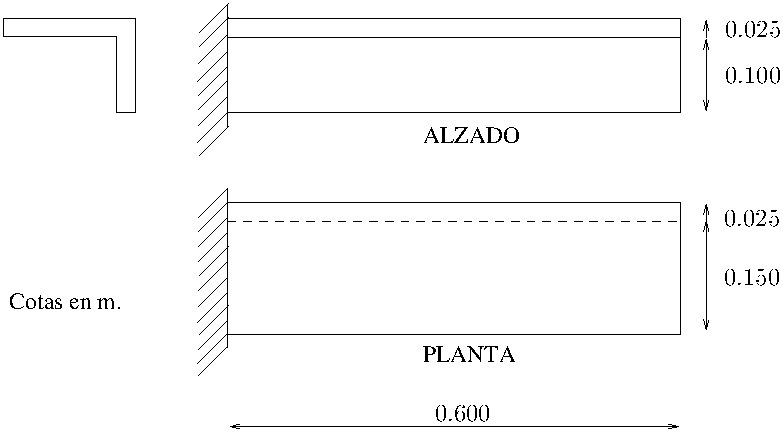
\includegraphics[width=0.7\textwidth]{ejerc3}
\end{center}

\vspace{5mm}



%\vspace{4mm}
%\begin{figure}[h]
%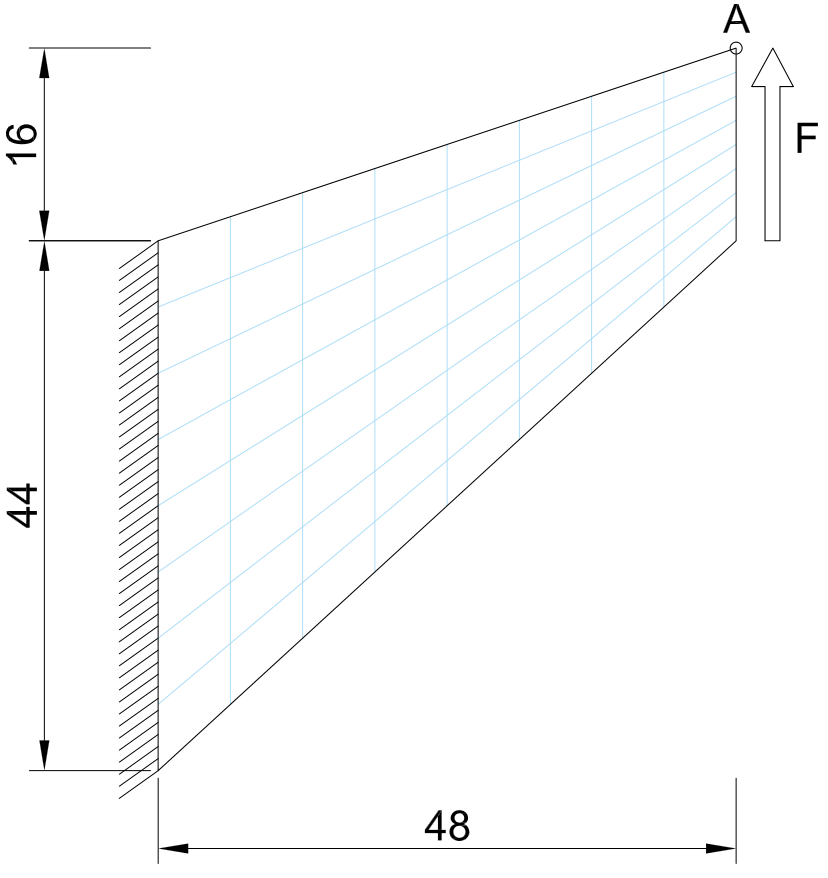
\includegraphics[width=10cm]{membrana8x8.png}
%\centering
%\end{figure}

\end{document}